\section{Auswertung}

Im Folgenden werden die erhobenen Messdaten ausgewertet, mit dem Ziel die Polarisation,
die Grundmode, sowie die erste Angeregte Mode, die Wellenlänge und die Stabilitätsmessung
des HeNe-Lasers zu erhalten.

\subsection{Polarisationsmessung}
\label{sec:pol}

Die Messdaten sind in Tab. \ref{tab:pol} dargestellt. Die Intensität $I(\varphi)$
ist in Abhängigkeit des Winkels des Polarisationsfilters $\varphi$ gemessen worden.

Die Messdaten sind an eine Funktion der Form:

\begin{equation}
  \label{eqn:Pol}
  I\left(\varphi\right) = I_0\cdot \sin^2\left(\varphi - \varphi_0\right)
\end{equation}

gefittet worden. Die einzelnen Parameter der Ausgleichsrechnung sind in Tab. \ref{tab:aus_pol}
dargestellt.

\begin{table}
\centering
\caption{Parameter der Ausgleichsrechnung zu \eqref{eqn:Pol}}
\label{tab:aus_pol}
\begin{tabular}{S S S}
\toprule
{Parameter} & {Wert} & {Fehler} \\
\midrule
$I_\text{0}$  & 0.26\text{mA} & 0.019 \\
$\varphi$ & 0.14\text{rad} & 0.067 \\
\bottomrule
\end{tabular}
\end{table}

\begin{figure}[h]
  \centering
  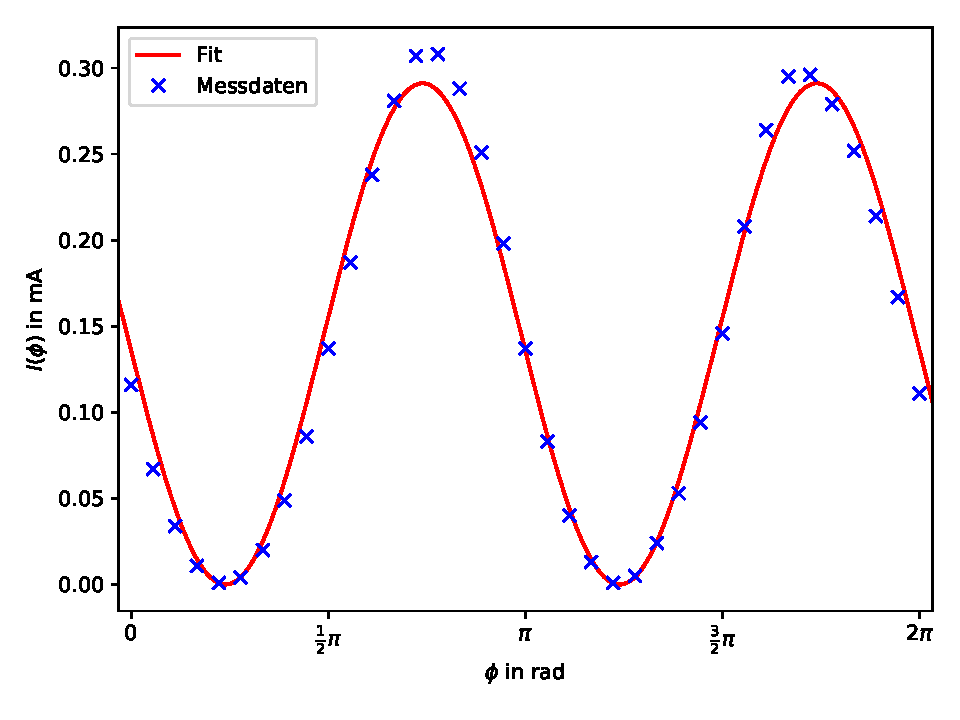
\includegraphics[width = \textwidth]{Pics/Polarisationsmessung.pdf}
  \caption{Polarisationsmessung mit der zugehörigen Ausgleichsfunktion.}
  \label{fig:Pol}
\end{figure}

\FloatBarrier

\subsection{Modenmessung}
\label{sec:tem}

Die Messdaten zu der Grundmode TEM$_{(0,0)}$ und der ersten angeregte Mode
TEM$_{(0,1)}$ sind in Tab. \ref{tab:tem} einzusehen.
Die Daten der Grundmode  an eine Gaußfunktion der Form:

\begin{equation}
  \label{eqn:gauß}
  I_{(0, 0)} = I_0\exp\left(-2\left(\frac{\Delta L - d_0}{\omega}\right)^2\right)
\end{equation}

gefittet worden.

\begin{figure}[h]
  \centering
  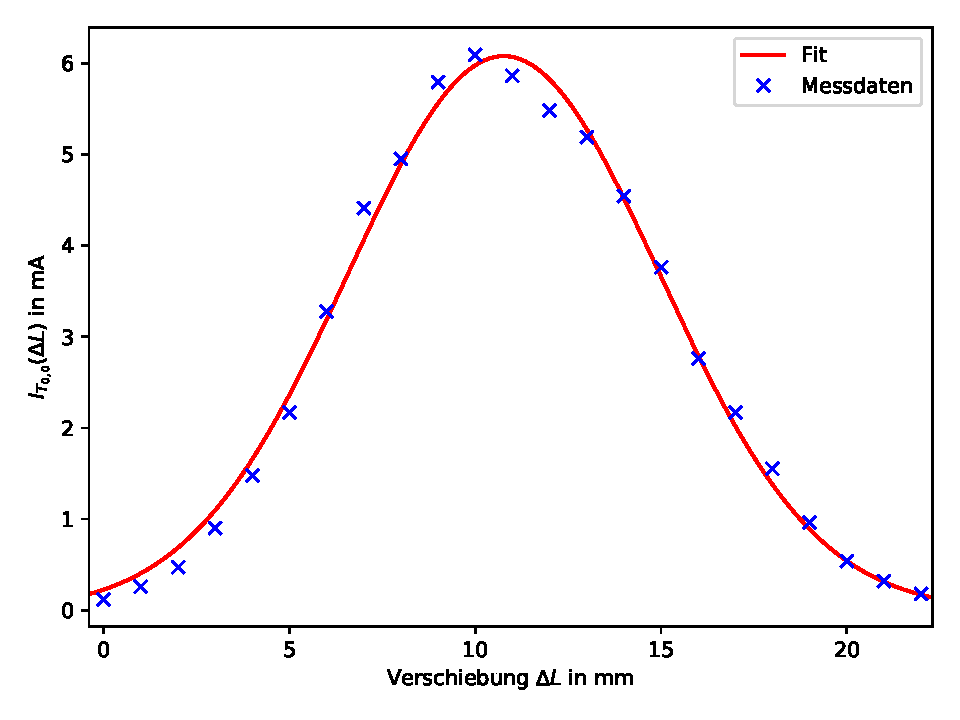
\includegraphics[width = \textwidth]{Pics/Grundmode.pdf}
  \caption{Grundmode mit der zugehörigen Ausgleichsfunktion.}
  \label{fig:Grundmode}
\end{figure}

Hingegen sind die Daten der TEM$_{(0,1)}$ an eine doppelte Gaußkurve
für asymmetrische Knotenlinien gefittet worden.
Die Ausgleichsfunktion besitzt folgenden Gestalt:

\begin{equation}
  \label{eqn:doppelter_gauß}
  I_{(0, 1)} = I_{0,1}\exp\left(-2\left(\frac{\Delta L - d_{0,1}}{\omega_1}\right)^2\right)
  + I_{0,2}\exp\left(-2\left(\frac{\Delta L - d_{0,2}}{\omega_2}\right)^2\right).
\end{equation}

Die Parameter der Ausgleichsrechnungen sind in Tab. \ref{tab:moden} aufgeführt.

\begin{table}
\centering
\caption{Parameter der Ausgleichsrechnung zu den Gleichungen \eqref{eqn:gauß} und \eqref{eqn:doppelter_gauß}}
\label{tab:moden}
\begin{tabular}{S S S}
\toprule
{Parameter} & {Wert} & {Fehler} \\
\midrule
$I_\text{0}$  & 6.08\text{mA} & 0.079 \\
$\Delta L_\text{0}$ & 10.77\text{mm} & 0.063 \\
$\omega$ & 8.396\text{mm} & 0.13 \\
$I_\text{0,1}$ & 0.65$\mu$\text{A} & 0.035 \\
$\Delta L_\text{0,1}$ & 4.68\text{mm} & 0.175 \\
$\omega_\text{1}$ & 5.63\text{mm} & 0.375 \\
$I_\text{0,2}$ & 0.45$\mu$\text{A} & 0.011 \\
$\Delta L_\text{0,2}$ & 18.61\text{mm} & 0.089 \\
$\omega_\text{2}$ & 6.46\text{mm} & 0.189 \\
\bottomrule
\end{tabular}
\end{table}

Mit der Funktion \eqref{eqn:doppelter_gauß} und den Parametern aus Tab. \ref{tab:moden}
ergibt sich die Ausgleichskurve zu dem in Abb. \ref{fig:moden} dargestellten Plot.

\begin{figure}[h]
  \centering
  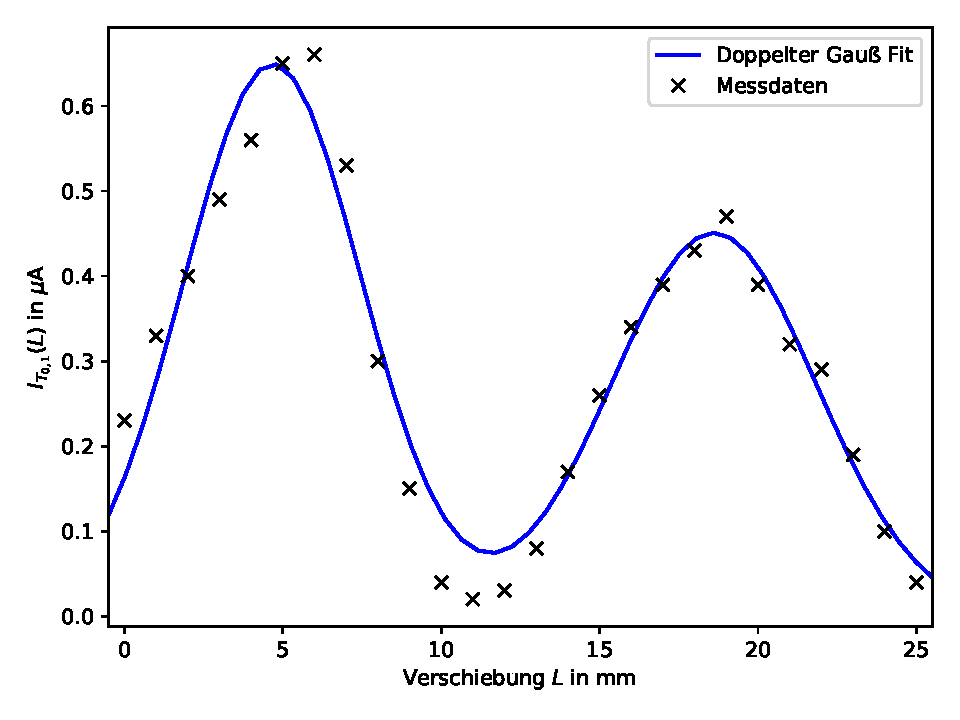
\includegraphics[width = \textwidth]{Pics/erste_angeregte_Mode.pdf}
  \caption{Erste angeregte Mode mit der zugehörigen Ausgleichsfunktion.}
  \label{fig:moden}
\end{figure}

\FloatBarrier

\subsection{Wellenlängenmessung}
\label{sec:wellenlänge}

Die Messdaten zu der Wellenlängenmessung ist in Tab. \ref{tab:wellenlänge}
dargestellt.
Die Wellenlänge wird durch Formel \eqref{eqn:wellenlänge} berechnet.

\begin{equation}
  \label{eqn:wellenlänge}
  \lambda = \frac{a\cdot\sin\left(\tan^-1\left(\frac{d_n}{L}\right)\right)}{n}
\end{equation}

Dabei ist $a$ die Gitterbreite, $d_n$ der Abstand der Hauptmaxima zu dem zentralen
Hauptmaxima, $L$ der Abstand des Schirms von dem Spalt und $n$ die Ordnung der
Hauptmaxima. Die Ordnung des Hauptmaximas wird wie in Abb. \ref{fig:ordnung}
dargestellt bestimmt.

\begin{figure}[h]
  \centering
  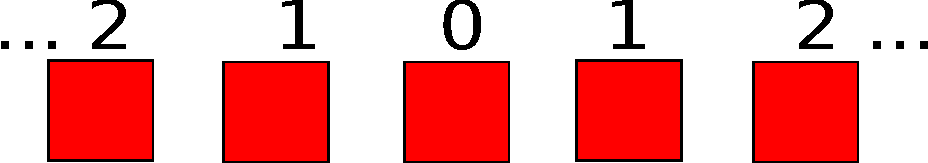
\includegraphics[width = 0.5\textwidth]{Pics/Ordnung.pdf}
  \caption{Schema zum Ablesen der Ordnung der Hauptmaxima.}
  \label{fig:ordnung}
\end{figure}

Dabei hat das zetrale Hauptmaxima die Ordnung 0.
Das verwendete Gitter hat eine Gitterbreite von $a = \frac{1}{100}\si{\milli\meter}$
und der Abstand zum Schirm beträgt $L = \SI{75.7}{\centi\meter}$. Als Ablesefehler
der Abstände der Hauptmaxima wird $\delta L = \SI{0.05}{\centi\meter}$ angenommen.

\begin{table}
\centering
\caption{Messdaten zur Wellenlängenmessung.}
\label{tab:wellenlänge}
\begin{tabular}{S S S @{${}\pm{}$} S}
\toprule
{Parameter} & {Wert in $\si{\centi\meter}$} & \multicolumn
{2}{c}{$\lambda$ in $\si{\nano\meter}$} \\
\midrule
$H_\text{-2}$  & 9.8 & 641.94 & 3.22 \\
$H_\text{-1}$ & 4.9 & 645.94  & 6.56 \\
$H_\text{1}$ & 5.1 & 672.18 & 6.56 \\
$H_\text{2}$ & 9.7 & 635.49 & 3.22 \\
\bottomrule
\end{tabular}
\end{table}

Gemittelt über die Anzahl ergeben die Wellenlängen
aus Tab. \ref{tab:wellenlänge} die beste Schätzung $\lambda\ua{He-Ne} = \SI{648.9(26)}{\nano\meter}$.

\FloatBarrier

\subsection{Stabilitätsmessung}
\label{sec:stabilitätsmessung}

Die Messdaten der Stabilitätsmessung des $\ce{He-Ne}$-Lasers für die verschiedenen
Resononatoren sind in in Tab. \ref{tab:kk} und Tab. \ref{tab:kp} dargestellt.

Die Messdaten des Resonators mit der Spiegelkombination konkav-konkav
sind an eine quadratische Funktion mit den Paramtern $a, b$ und $c$ gefittet (vgl. \eqref{eqn:quad}).

\begin{equation}
  \label{eqn:quad}
  I\ua{quad}\left(\Delta L\right) = a\cdot\left(\Delta L\right)^2 + b\cdot\Delta L + c
\end{equation}

Aus der Ausgleichsrechnung ergeben sich die Parameter zu:

\begin{align}
  \label{eqn:params_kk}
  a =& \SI{-7.68(928)e-6}{\milli\ampere\per\centi\meter^2}\\
  b =& \SI{3.57(175)e-3}{\milli\ampere\per\centi\meter}\\
  c =& \SI{-6.83(807)e-2}{\milli\ampere}.
\end{align}

Hingegen werden die Messdaten des Resonators mit der Spiegelkombination konkav-planar
an eine lineare Funktion mit den Parametern $a$ und $b$ gefittet (vgl. \eqref{eqn:lin}).

\begin{equation}
  \label{eqn:lin}
  I\ua{lin}\left(\Delta L\right) = a\cdot\Delta L + b
\end{equation}

Die Parameter der Ausgleichsrechnung der Funktion \eqref{eqn:lin} ergeben sich zu:

\begin{align}
  \label{eqn:params_kp}
  a =& \num{-6.71(89)e-2}\frac{\mu\si{\ampere}}{\si{\centi\meter}}\\
  b =& \num{6.52(61)}\mu\si{\ampere}
\end{align}

Die dazugehörigen Diagramme sind in Abb. \ref{fig:stabilität_quad} und Abb. \ref{fig:stabilität_lin}
dargestellt.

\begin{figure}[h]
  \centering
  \includegraphics[width = \textwidth]{Pics/Stabilität_kk.pdf}
  \caption{Messdaten und Fit der Stabilitätsmessung des Resonators mit der Spiegelkombination konkav-konkav.}
  \label{fig:stabilität_quad}
\end{figure}

\begin{figure}[h]
  \centering
  \includegraphics[width = \textwidth]{Pics/Stabilität_kp.pdf}
  \caption{Messdaten und Fit der Stabilitätsmessung des Resonators mit der Spiegelkombination konkav-planar.}
  \label{fig:stabilität_lin}
\end{figure}

\section{Diskussion}

In diesem Kapitel werden die Messergebnisse diskutiert.
Der Zusammenhang der Polarisationsmessung mit einer
quadrierten Sinusfunktion ist deutlich erkennbar. Somit konnte die Erwartung durch
die Messung bestätigt  werden.
Weiterhin sind die Grundmode und die erste angeregte Mode ausgemessen worde.
Die Grundmode konnte der Erwartung entsprechend durch eine Gaußfunktion präzise beschrieben werden.
Die erste angeregte Mode wird hingegen durch eine asymmetrische doppelte Gaußfunktion
beschrieben. Die Asymmetrie entsteht aufgrund der endlichen Ausdehnung des verwendeten
Golddrahtes. Der Golddraht wirft auf die eine Seite der doppelten Gaußfunktion einen
Schatten, der das Maximum deutlich absenkt.

Die Wellenlängenmessung ergibt $\lambda\ua{He-Ne} = \SI{648.9(26)}{\nano\meter}$.
Dieser Wert liegt im roten Bereich des sichtbaren Lichtes. Der Literaturwert wird
mit $\lambda\ua{lit} = \SI{632,82}{\nano\meter}$. Die Dieskrepanz der beiden Werte liegt
nicht im Fehlerintervall des experimentell bestimmten Wertes. Dies kann dadurch erklärt
werden, dass der Schirm, auf den die Hauptmaxima projeziert werden schief gestanden
haben könnte. Außerdem ist die Vermessung und Rechnung im Nanometer Bereich anfällig
für Ablesefehler. Daher wird die Diskrepanz auf einen systematischen Fehler
zurückgeführt.

Die Stabilitätsmessung ergab, dass ein Zusammenhang zwischen der konkav-konkav
Resonatorspiegelkombination und einer quadratischen Gleichung hergestellt werden
konnte. Die Parameter der Auslgeichsrechnung haben jedoch große statistische
Unsicherheiten, aber der Zusammenhang wird trotzdem ersichtlich.
Ebenso ist der lineare Zusammenhang der konkav-planar Resonatorspiegelkombination
in dem Kapitel \ref{sec:stabilitätsmessung} aufgeführt worde.
Das konkav-planar System stellt bei der Vermessung deutlich Probleme dar, weil
der $\ce{He-Ne}$-Laser schon bei kleinen Spiegelveränderungen aufgehört hat zu lasern.
Die Messung wurde mehrfach druchgeführt, da die Messreihen teilweise schon nach zwei
Messpunkten abgeborchen sind, weil der Laser bei gegebenen Abstand nicht mehr zum lasern gebracht werden
konnte. Letztendlich sind nur fünf Messpunkte aufgenommen worden, weshlab das
Ergebnis starke statistische Unsicherheiten aufweist.

\section{Messdaten}

In diesem Kapitel sind die Messdaten zu den Kapiteln \ref{sec:pol}, \ref{sec:tem}
und \ref{sec:stabilitätsmessung} aufgeführt.


\begin{table}
\centering
\caption{Messdaten der Polarisationsmessung.}
\label{tab:pol}
\begin{tabular}{S S}
\toprule
{$I\ua{Pol}$ in $\si{\milli\ampere}$} & {$\phi$ in  $\si{\degree}$}  \\
\midrule
0.116  & 0\\
0.067  & 10\\
0.034  & 20\\
0.011  & 30\\
0.001  & 40\\
0.004  & 50\\
0.020  & 60\\
0.049  & 70\\
0.086  & 80\\
0.137  & 90\\
0.187  & 100\\
0.238  & 110\\
0.281  & 120\\
0.307  & 130\\
0.308  & 140\\
0.288  & 150\\
0.251  & 160\\
0.198  & 170\\
0.137  & 180\\
0.083  & 190\\
0.040  & 200\\
0.013  & 210\\
0.001  & 220\\
0.005  & 230\\
0.024  & 240\\
0.053  & 250\\
0.094  & 260\\
0.146  & 270\\
0.208  & 280\\
0.264  & 290\\
0.295  & 300\\
0.296  & 310\\
0.279  & 320\\
0.252  & 330\\
0.214  & 340\\
0.167  & 350\\
0.111  & 360\\
\bottomrule
\end{tabular}
\end{table}

\begin{table}
\centering
\caption{Messdaten der Modenmessung.}
\label{tab:tem}
\begin{tabular}{S S S }
\toprule
{$I_{(0, 0)}$ in $\mu\si{\ampere}$} & {$I_{(0, 1)}$ in $\mu\si{\ampere}$} & {$\Delta L$ in $\si{\milli\meter}$}  \\
\midrule
0.12  & 0.23  & 0\\
0.26  & 0.33  & 1\\
0.47  & 0.40  & 2\\
0.90  & 0.49  & 3\\
1.48  & 0.56  & 4\\
2.17  & 0.65  & 5\\
3.28  & 0.66  & 6\\
4.41  & 0.53  & 7\\
4.95  & 0.30  & 8\\
5.79  & 0.15  & 9\\
6.09  & 0.04  & 10\\
5.86  & 0.02  & 11\\
5.48  & 0.03  & 12\\
5.19  & 0.08  & 13\\
4.54  & 0.17  & 14\\
3.76  & 0.26  & 15\\
2.76  & 0.34  & 16\\
2.17  & 0.39  & 17\\
1.55  & 0.43  & 18\\
0.96  & 0.47  & 19\\
0.54  & 0.39  & 20\\
0.32  & 0.32  & 21\\
0.18  & 0.29  & 22\\
\text{\,\,\,\,\,\,\,\,\,\,\,\,\,\,\,\,--}  & 0.19  & 23\\
\text{\,\,\,\,\,\,\,\,\,\,\,\,\,\,\,\,--}  & 0.10  & 24\\
\text{\,\,\,\,\,\,\,\,\,\,\,\,\,\,\,\,--}  & 0.04  & 25\\
\bottomrule
\end{tabular}
\end{table}

\begin{table}
\centering
\caption{Messdaten der Resonatorstabilitätemessung für die Spiegelkombination konkav-konkav.}
\label{tab:kk}
\begin{tabular}{S S}
\toprule
{$\Delta L$ in $\si{\centi\meter}$} & {$I$ in $\si{\milli\ampere}$}  \\
\midrule
67.0  & 0.14\\
72.3  & 0.14\\
77.1  & 0.16\\
82.0  & 0.17\\
87.1  & 0.18\\
91.7  & 0.21\\
97.1  & 0.21\\
102.1  & 0.22\\
107.0  & 0.21\\
112.1  & 0.23\\
122.1  & 0.26\\
\bottomrule
\end{tabular}
\end{table}

\begin{table}
\centering
\caption{Messdaten der Resonatorstabilitätemessung für die Spiegelkombination konkav-planar.}
\label{tab:kp}
\begin{tabular}{S S}
\toprule
{$\Delta L$ in $\si{\centi\meter}$} & {$I$ in $\si{\micro\ampere}$}  \\
\midrule
58.9  & 2.57\\
62.9  & 2.40\\
68.1  & 1.83\\
73.1  & 1.48\\
78.1  & 1.40\\
\bottomrule
\end{tabular}
\end{table}

